
%\documentclass[10pt]{phdsymp} %!PN
\documentclass[9pt, twocolumn]{phdsymp} %!PN
%\documentclass[12pt,draft]{phdsymp} %!PN
%\documentstyle[twocolumn]{phdsymp}
%\documentstyle[12pt,twoside,draft]{phdsymp}
%\documentstyle[9pt,twocolumn,technote,twoside]{phdsymp}

\usepackage[english]{babel}       % Voor nederlandstalige hyphenatie (woordsplitsing)
\usepackage{hyperref}
\usepackage{graphicx}                   % Om figuren te kunnen verwerken
\usepackage{graphics}			% Om figuren te verwerken.
\graphicspath{{figuren/}}               % De plaats waar latex zijn figuren gaat halen.

\usepackage{times}

\hyphenation{si-mu-la-ted re-a-lis-tic packets really in-clu-ding}

\def\BibTeX{{\rm B\kern-.05em{\sc i\kern-.025em b}\kern-.08em
    T\kern-.1667em\lower.7ex\hbox{E}\kern-.125emX}}

\newtheorem{theorem}{Theorem}

\begin{document}

\title{Identifying experts through a framework for knowledge extraction from public online sources} %!PN

\author{Simon Buelens and Mattias Putman}

\supervisor{Prof. Dr. Ir. Filip De Turck, Dr. Ir. Elena Tsiporkova, Dr. Ir. Tom Tourw\'e, Ir. Anna Hristoskova, Ir. Tim Wauters}

\maketitle

\begin{abstract} 

Researchers are losing too much valuable time searching for related research material. There are only few services out there that offer a keyword-based search for retrieving experts. The goal of this article is the creation of a framework that retrieves information from online sources, combines the information based on author and gives the authors a ranking based on the level of expertise for a certain keyword or keyphrase. The article starts from a theoretical point of view, defining the optimal manner of execution. Afterwards, the actual implementation is thoroughly explained, which makes use of a graph representation and pipes and filters. The clustering process, responsible for linking the names to the actual authors, is one of the key components. The article ends with a comparative analysis of the results.

\end{abstract}

\begin{keywords}
author disambiguation, data processing, clustering, pipes and filters
\end{keywords}

\section{Introduction}

Researchers lose valuable time searching for research material related to their field of expertise. The process of finding and verifying experts is extensive and troublesome. The aim of this article is creating a framework that is capable of retrieving publications and related information from online sources, analyzing this information and linking it to the correct author and enabling users to search for experts for a given subject. The main focus is on the disambiguation of authors, the classification into clusters and the extensibility of the framework.

\begin{figure}[h!]
	\centering
	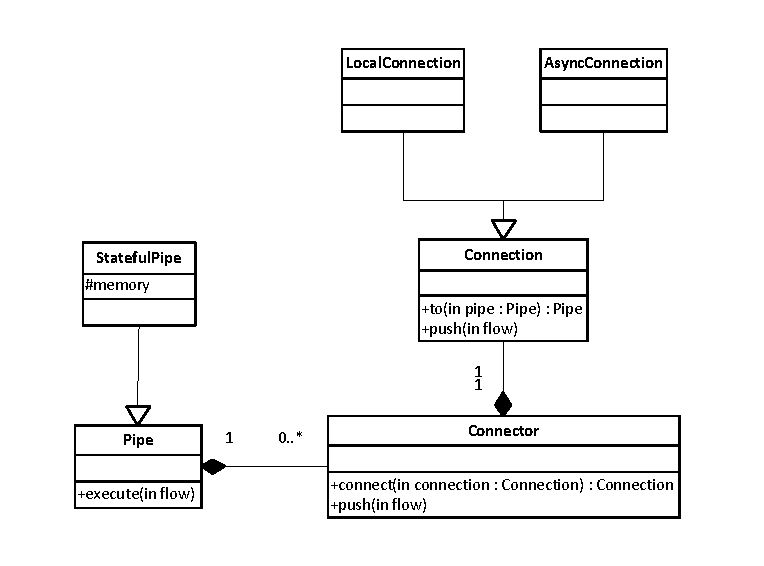
\includegraphics[width= 0.38\textwidth]{fig/architecturev2.pdf}
	\caption{The architecture: pipes and filters.}
	\label{fig:arch}
\end{figure}

\section{Theoretical Model}

The foundation of the framework is based on the five following observations:

\begin{enumerate}
	\item All instances are different authors until proven otherwise.
	\item No decision is made permanent.
	\item Any information is considered partial information.
	\item A constantly changing input asks for a constantly changing output.
	\item The stream of information is endless.
\end{enumerate}

Starting from this foundation, the article lays out the rudiments of the framework, starting with a theoretical model. This model is composed of three layers, combining the structural, informational and algorithmic aspects that emerge from dealing with the difficulties related to author disambiguation. This is achieved by a graph representation where the authors are phased in three different levels. At the highest level is the family name, below are authors that are considered unique (a cluster) containing instances of names that are linked to the publications. This allows name-matching and regrouping without losing information.

The theoretical model also contains a summary of the different rules. They drive the entire flow of the framework by converting new information into similarities between instances. The four rules that are examined are:

\begin{description}
	\item[- Community Rule] Exploiting the fact that authors often work together with the same co-author. \autoref{fig:coauthor} gives a visual representation of how this works.
	\item[- Interest Rule] The subjects of publications of the same author are usually located within the same field of research.
	\item[- Email Rule] Authors with the same email address, are most likely the same person.
	\item[- Affiliation Rule] Authors are more likely to work at one affiliation at a given time.
\end{description}

\begin{figure}[ht!]
	\centering
	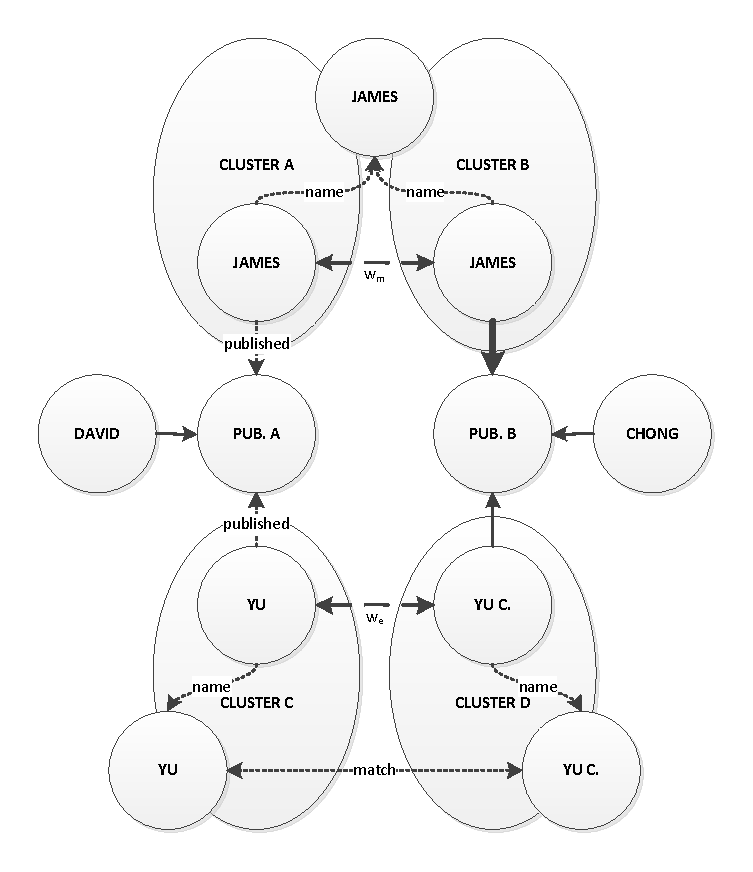
\includegraphics[width= 0.38\textwidth]{fig/coauthorrulenameeq.pdf}
	\caption{The co-author rule in action: comparing the two instance of James, a similarity ($w_m$) is added as the co-authors Yu and Yu C. match.}
	\label{fig:coauthor}
\end{figure}

Rules are triggered by different events in the system. A rule could for example be executed when it has been discovered that an instance has published a publication, but could be executed on the event of a reclustering as well. The latter is a message that is a byproduct of the system itself and not originating from an external source.

Rules can be performed on three different scopes: instances with the same name, instances with similar names and instances part of the same cluster. That means that the instances of those collections are compared with the concerning instance. Strictly respecting this scopes narrow down the problem domain.

\section{Pipes and Filters}
\label{pipes}

The core of the implementation of the framework is the simplicity achieved by pipes and filters. The architecture is shown in \autoref{fig:arch}. They allow for modifiability and extensibility as pipes processing new sources or calculating new similarities between instances can easily be added to the system. An overview of the different pipes and the flow that runs between them is shown on \autoref{fig:pipes}. The expressiveness of StatefulPipe and the scalability of AsyncConnection in combination with a shared key-value store enables out-of-the-box and carefree scalability.

\begin{figure}[hb!]
	\centering
	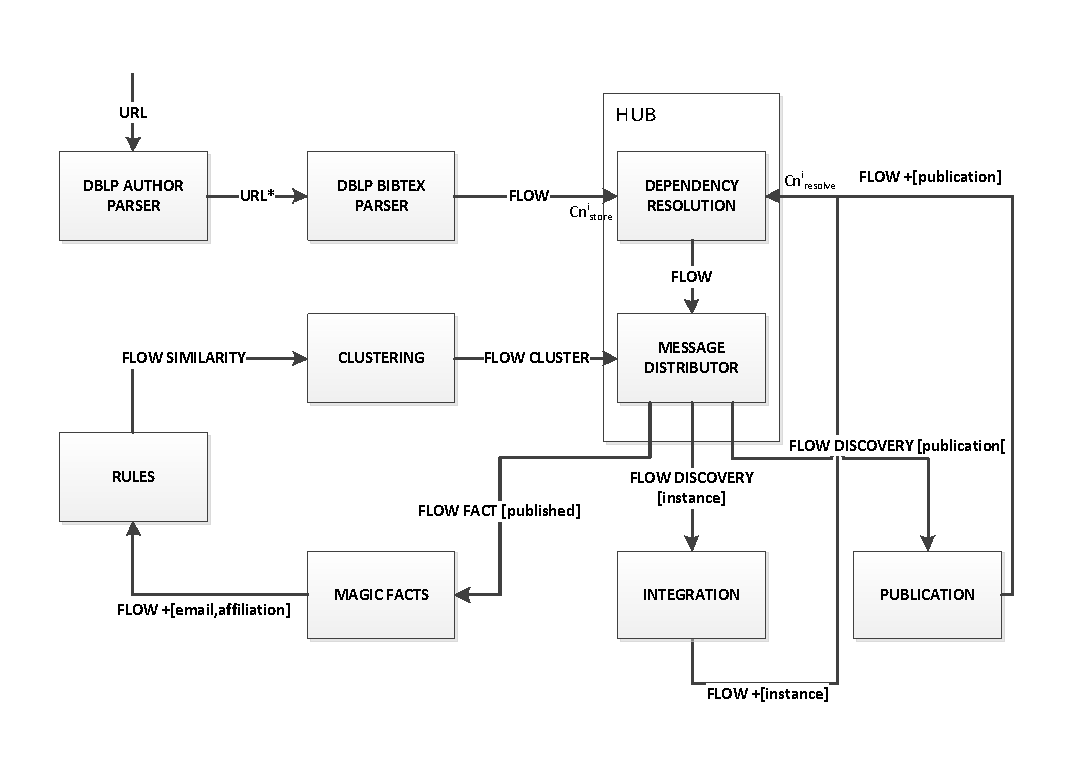
\includegraphics[width= 0.38\textwidth]{fig/completepipesmall.pdf}
	\caption{An overview of the different pipes and the flow running between them.}
	\label{fig:pipes}
\end{figure}

\section{Clustering}
The article focuses a lot on the clustering process. This process is responsible for calculating what instances match to the same author, based on similarities between the instances. Every time a rule computes a new similarity, it is possible reclustering has to occur. As there is a constant influx of information, there is a need for a dynamic approach that maintains the cluster quality. 

The article gives an in-depth explanation of the dynamic clustering algorithm described in \cite{dynamic}. The algorithm itself depends on the minimum cut tree algorithm. The sequential Gusfield's algorithm described in \cite{gusfield} is implemented. 

The article also proposes an addition to the original clustering algorithm. It introduces a new case, acting the same as case 1, but being executed instead of case 3 on the occasion that $2 * \frac{cutvalue(C_v, C_u)}{\left|V\right|} <= \alpha / 2$. This anticipates the fact that a lot of similarities with lower weights occur and they often take place in succession. Often this results in case 3 being calculated multiple times in succession, before finally merging the clusters together. By introducing this new case, the resource-intensive execution of case 3 is swapped for the very fast execution of case 1.

The clustering process is implemented as a stateful pipe and is not treated any different from the other pipes. The clustering process is completely decoupled from the graph representation. Better yet, the graph is almost not being accessed during the clustering process. The reasoning about the grouping of instances is done completely local and the state of the similarities (the similarity plane) is maintained in the shared key-value store. This approach takes a lot of load off the database, which is important as a graph database does not scale that easily.

\section{Results}

The proposed framework is tested against a manually annoted dataset containing over 1000 publications. The impact of each of the rules on the accuracy is tested and the combination of the four rules is concluded as having the highest overall accuracy. The co-author rule has the biggest positive impact on the correctness. The F measure is also calculated for different distributions of the weights for each of the rules. The distribution giving favor to a lot of clustering by setting all the values high and the alpha value just a little higher, renders the best results. 

In the article, there is also a comparison between the results the proposed framework gets and the accuracy of DBLP. The conclusion is that the proposed framework overcomes DBLP by $14\%$ or $17\%$, depending on how the mean accuracy is calculated.


\begin{figure}[htpb!]
\centering
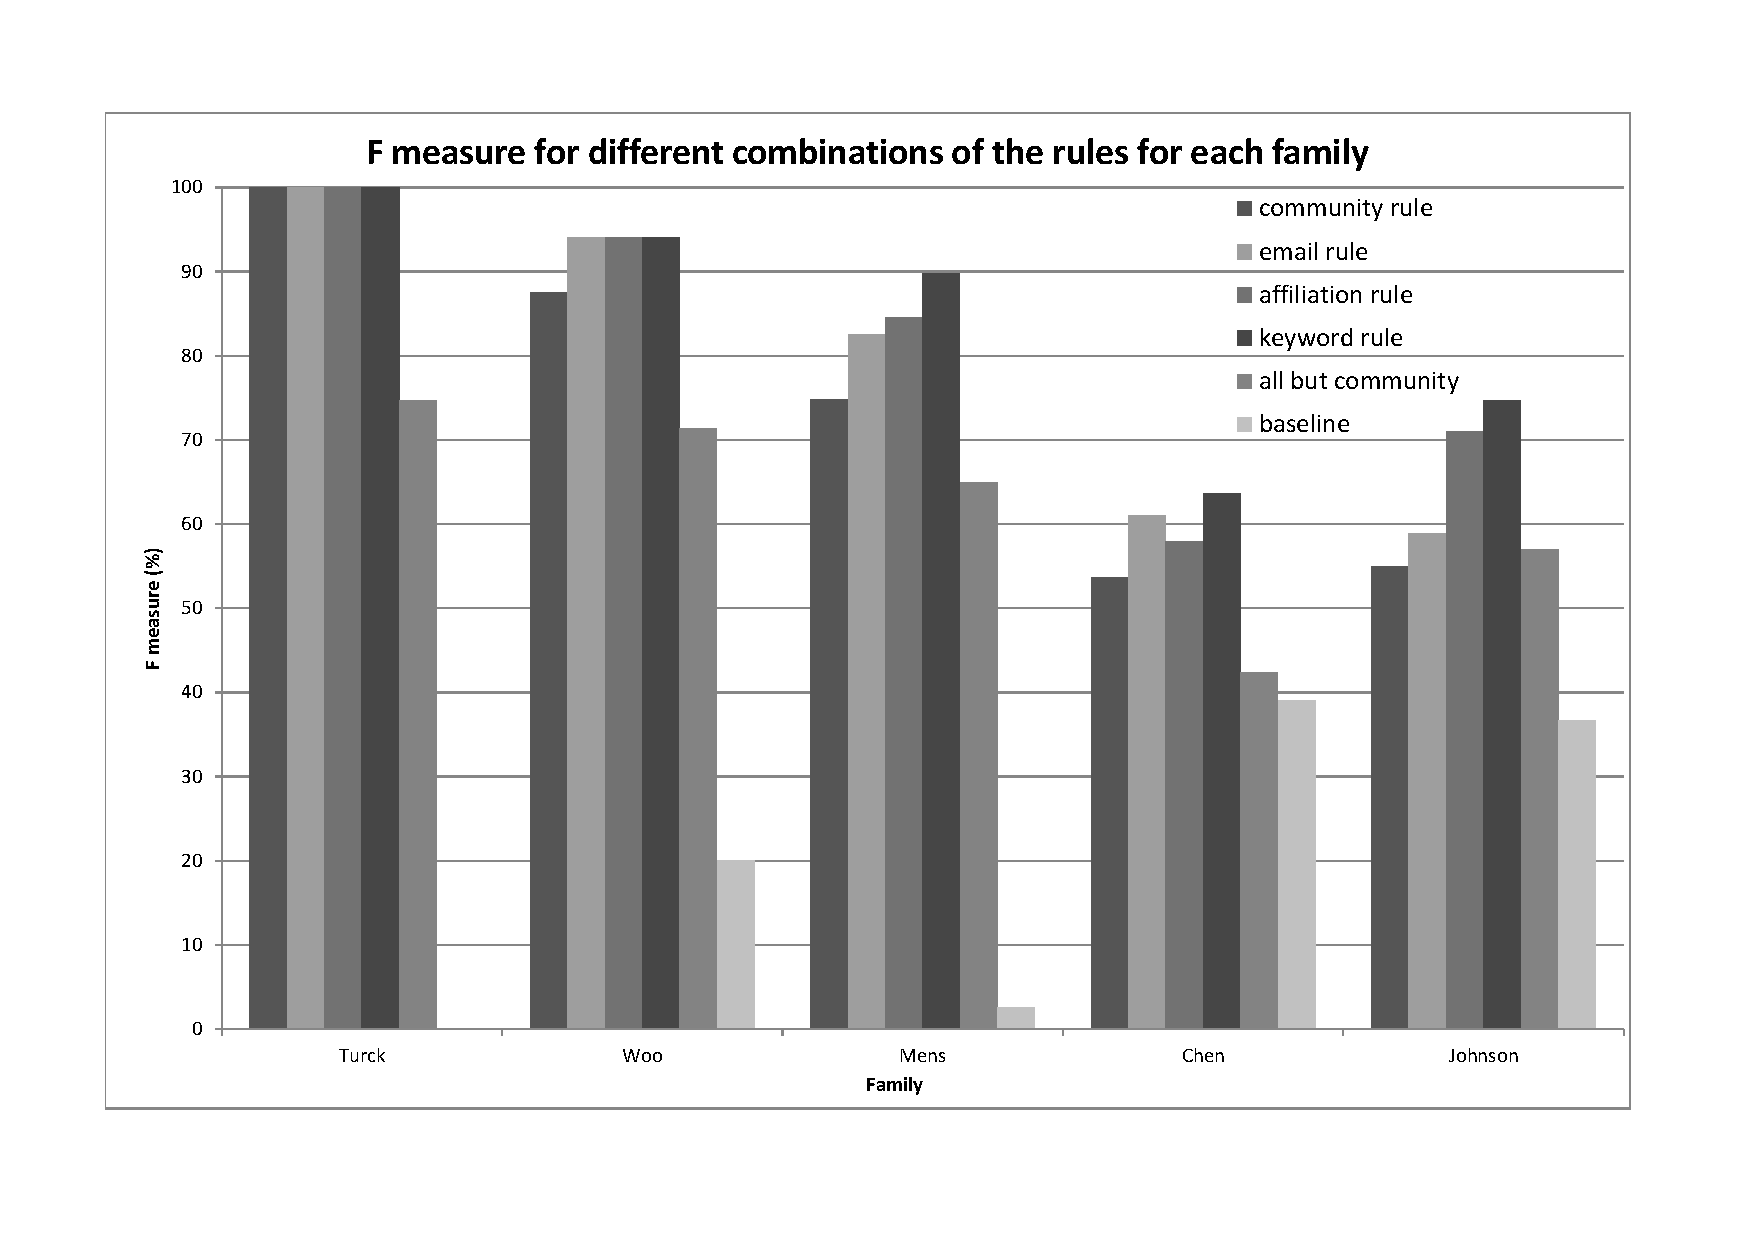
\includegraphics[width= 0.45\textwidth]{fig/test-rules.pdf}
\caption{A comparison of different combinations of rules. The first four columns stack the rules, the fifth column uses all rules except the community rule and the last column depicts the base line, this is the F measure of the case where no clustering has happened.}
\label{fig:testperformance}
\end{figure}

\section{Conclusions and future work}

This article examined the opportunities using the semantic web and data processing. The possibilities within expert finding and author disambiguation are challenging and can contribute in solving a real-life problem. A framework has been composed, focusing on author disambiguation by implementing a dynamic clustering algorithm, allowing for real-time applications. The proposed extensibility has been accomplished by the usage of pipes and filters.

The results show that the framework is able to improve the results from DBLP. However, there is still room for more improvements. The most important additions would be enabling the usage of negative weights and adding more online sources in order to retrieve more information about the authors. This extra information could also entail the addition of new rules, but, as stated before, pipes make this an easy task.


%\nocite{*}
\bibliographystyle{phdsymp}
%%%%%\bibliography{bib-file}  % commented if *.bbl file included, as
%%%%%see below


%%%%%%%%%%%%%%%%% BIBLIOGRAPHY IN THE LaTeX file !!!!! %%%%%%%%%%%%%%%%%%%%%%%%
%% This is nothing else than the phdsymp_sample2e.bbl file that you would%%
%% obtain with BibTeX: you do not need to send around the *.bbl file        
%%
%%---------------------------------------------------------------------------%%
%
\begin{thebibliography}{1}
%\bibitem{paper}
%Bart Lannoo, Didier Colle, Mario Pickavet, Piet Demeester,
%\newblock {\em Optical Switching Architecture to Implement Moveable Cells in a Multimedia Train Environment},
%\newblock Proc. of ECOC 2004, 30th European Conf. on Optical Communication, vol. 3, pp. 344-345, Stockholm, Sweden, 5-9 Sep. 2004.
%
\bibitem{dynamic}
Saha B., Mitra P. \newblock{\em Dynamic algorithm for graph clustering using minimum cut tree} 2006. 

\bibitem{gusfield}
Flake G.W., Tarjan R.E., Tsioutsiouliklis K. \newblock{\em Graph clustering and minimum cut trees} 2004

%
%\bibitem{click}
%\newblock {\em The Click Modular Router Project},
%\newblock http://www.read.cs.ucla.edu/click/
%
%\bibitem{ns}
%\newblock {\em {NS} -- {N}etwork {S}imulator},
%\newblock http://nsnam.isi.edu/nsnam/
\end{thebibliography}
%
%%---------------------------------------------------------------------------%%

\end{document}

%%%%%%%%%%%%%%%%%%%%%  End of phdsymp_sample2e.tex  %%%%%%%%%%%%%%%%%%%%%%%%%%%
